\documentclass[12pt, a4paper]{article}
\usepackage[utf8]{inputenc}
\usepackage{geometry}
\usepackage{graphicx}
\usepackage{tikz}
\usepackage{tabularx}
\usepackage{multicol}
\usepackage{multirow}
\usepackage{array,booktabs,ragged2e}
\usepackage{amsmath}
\usepackage{xkeyval}
\usepackage{float}
\usepackage{physics}
\usepackage{tfrupee}
\usepackage{mathtools} %underbrace symbol
\usepackage{adjustbox} 
\usepackage{xcolor}
\usepackage{colortbl}
\usepackage{tkz-euclide}
\usepackage{pgf-pie}
\usepackage[misc]{ifsym} %Used in tally mark
\usetikzlibrary{patterns,calc}

\newcommand{\scalefactor}{1}


\geometry{top=2.5cm, bottom=1.25cm, left=1.5cm, right=1.5cm}
\makeatletter
%-----------------------------------------------------------
% text bottom 4 option in 1 row
%-----------------------------------------------------------

\define@key{mcqtextbottomFourOne}{questionnumber}{\def\mcqtextbottomFourOnequestionnumber{#1}} 
\define@key{mcqtextbottomFourOne}{questionTag}{\def\mcqtextbottomFourOnequestionTag{#1}}
\define@key{mcqtextbottomFourOne}{questiontext}{\def\mcqtextbottomFourOnequestiontext{#1}}
\define@key{mcqtextbottomFourOne}{optionA}{\def\mcqtextbottomFourOneoptionA{#1}}
\define@key{mcqtextbottomFourOne}{optionB}{\def\mcqtextbottomFourOneoptionB{#1}}
\define@key{mcqtextbottomFourOne}{optionC}{\def\mcqtextbottomFourOneoptionC{#1}}
\define@key{mcqtextbottomFourOne}{optionD}{\def\mcqtextbottomFourOneoptionD{#1}}
\define@key{mcqtextbottomFourOne}{correctoption}{\def\mcqtextbottomFourOnecorrectoption{#1}}


\newcommand{\mcqtextbottomFourOne}[1]{%
\setkeys{mcqtextbottomFourOne}{#1}%
\vspace{2.5mm}
\begin{raggedright}
\textbf{Question Tag:} \mcqtextbottomFourOnequestionTag \hfill \textbf{Correct Option:} \mcqtextbottomFourOnecorrectoption\\
\end{raggedright}
\vspace{\baselineskip}
\begin{raggedright}
\textbf{Question \mcqtextbottomFourOnequestionnumber:} \mcqtextbottomFourOnequestiontext\\
\medskip
(a) \medskip \mcqtextbottomFourOneoptionA\\
(b) \medskip \mcqtextbottomFourOneoptionB\\      
(c) \medskip \mcqtextbottomFourOneoptionC\\
(d) \medskip \mcqtextbottomFourOneoptionD\\
\end{raggedright}
}

%-----------------------------------------------------------

%-----------------------------------------------------------

% DEFINE KEY FOR mcqtextbottomOneFour %

\define@key{mcqtextbottomOneFour}{questionnumber}{\def\mcqtextbottomOneFourquestionnumber{#1}} 
\define@key{mcqtextbottomOneFour}{questiontext}{\def\mcqtextbottomOneFourquestiontext{#1}}
\define@key{mcqtextbottomOneFour}{optionA}{\def\mcqtextbottomOneFouroptionA{#1}}
\define@key{mcqtextbottomOneFour}{optionB}{\def\mcqtextbottomOneFouroptionB{#1}}
\define@key{mcqtextbottomOneFour}{optionC}{\def\mcqtextbottomOneFouroptionC{#1}}
\define@key{mcqtextbottomOneFour}{optionD}{\def\mcqtextbottomOneFouroptionD{#1}}
\define@key{mcqtextbottomOneFour}{questionTag}{\def\mcqtextbottomOneFourquestionTag{#1}} 
\define@key{mcqtextbottomOneFour}{correctoption}{\def\mcqtextbottomOneFourcorrectoption{#1}}

% COMMAND FOR mcqtextbottomOneFour %

\newcommand{\mcqtextbottomOneFour}[1]{%
\setkeys{mcqtextbottomOneFour}{#1}%
\vspace{2.5mm}
\begin{raggedright}
\textbf{Question Tag:} \mcqtextbottomOneFourquestionTag \hfill \textbf{Correct Option:} \mcqtextbottomOneFourcorrectoption\\
\end{raggedright}
\vspace{\baselineskip}
\begin{raggedright}
\textbf{Question \mcqtextbottomOneFourquestionnumber:} \mcqtextbottomOneFourquestiontext
\begin{multicols}{4}
(a) \medskip \mcqtextbottomOneFouroptionA\\
(b) \medskip \mcqtextbottomOneFouroptionB\\      
(c) \medskip \mcqtextbottomOneFouroptionC\\
(d) \medskip \mcqtextbottomOneFouroptionD\\
\end{multicols}
\end{raggedright}
}

%-----------------------------------------------------------

%-----------------------------------------------------------

% Define key FOR mcqtextbottomOneTwo 

\define@key{mcqtextbottomOneTwo}{questionnumber}{\def\mcqtextbottomOneTwoquestion{#1}}
\define@key{mcqtextbottomOneTwo}{questiontext}{\def\mcqtextbottomOneTwoquestiontext{#1}}
\define@key{mcqtextbottomOneTwo}{optionA}{\def\mcqtextbottomOneTwooptionA{#1}}
\define@key{mcqtextbottomOneTwo}{optionB}{\def\mcqtextbottomOneTwooptionB{#1}}
\define@key{mcqtextbottomOneTwo}{questionTag}{\def\mcqtextbottomOneTwoquestionTag{#1}}
\define@key{mcqtextbottomOneTwo}{correctoption}{\def\mcqtextbottomOneTwocorrectoption{#1}}

% COMMAND FOR mcqtextbottomOneTwo %

\newcommand{\mcqtextbottomOneTwo}[1]{%
\setkeys{mcqtextbottomOneTwo}{#1}%
\vspace{2.5mm}
\begin{raggedright}
\textbf{Question Tag:} \mcqtextbottomOneTwoquestionTag \hfill \textbf{Correct Option:} \mcqtextbottomOneTwocorrectoption\\
\end{raggedright}
\vspace{\baselineskip}
\begin{raggedright}
\textbf{Question \mcqtextbottomOneTwoquestion:} \mcqtextbottomOneTwoquestiontext\\
\begin{multicols}{2}
(a) \medskip \mcqtextbottomOneTwooptionA\\
(b) \medskip \mcqtextbottomOneTwooptionB\\
\end{multicols}
\end{raggedright}
}

%-----------------------------------------------------------

%-----------------------------------------------------------

% Define key FOR mcqtextbottomTwoTwo

\define@key{mcqtextbottomTwoTwo}{questionnumber}{\def\mcqtextbottomTwoTwoquestion{#1}}
\define@key{mcqtextbottomTwoTwo}{questiontext}{\def\mcqtextbottomTwoTwoquestiontext{#1}}
\define@key{mcqtextbottomTwoTwo}{optionA}{\def\mcqtextbottomTwoTwooptionA{#1}}
\define@key{mcqtextbottomTwoTwo}{optionB}{\def\mcqtextbottomTwoTwooptionB{#1}}
\define@key{mcqtextbottomTwoTwo}{optionC}{\def\mcqtextbottomTwoTwooptionC{#1}}
\define@key{mcqtextbottomTwoTwo}{optionD}{\def\mcqtextbottomTwoTwooptionD{#1}}
\define@key{mcqtextbottomTwoTwo}{questionTag}{\def\mcqtextbottomTwoTwoquestionTag{#1}}
\define@key{mcqtextbottomTwoTwo}{correctoption}{\def\mcqtextbottomTwoTwocorrectoption{#1}}

% COMMAND FOR mcqtextbottomTwoTwo %

\newcommand{\mcqtextbottomTwoTwo}[1]{%
\setkeys{mcqtextbottomTwoTwo}{#1}%
\vspace{1.5mm}
\begin{raggedright}
\textbf{Question Tag:} \mcqtextbottomTwoTwoquestionTag \hfill \textbf{Correct Option:} \mcqtextbottomTwoTwocorrectoption\\
\end{raggedright}
\vspace{\baselineskip}
\begin{raggedright}
\textbf{Question \mcqtextbottomTwoTwoquestion:} \mcqtextbottomTwoTwoquestiontext\\
\begin{multicols}{2}
(a) \medskip \mcqtextbottomTwoTwooptionA\\
(c) \medskip \mcqtextbottomTwoTwooptionC\\
\columnbreak
(b) \medskip \mcqtextbottomTwoTwooptionB\\
(d) \medskip \mcqtextbottomTwoTwooptionD\\
\end{multicols}
\end{raggedright}
\vspace{5mm}
}

%-----------------------------------------------------------

%-----------------------------------------------------------

% Define key FOR mcqtextsideFourOne


\define@key{mcqtextsideFourOne}{questionnumber}{\def\mcqtextsideFourOnequestionnumber{#1}} 
\define@key{mcqtextsideFourOne}{questionTag}{\def\mcqtextsideFourOnequestionTag{#1}} 
\define@key{mcqtextsideFourOne}{questiontext}{\def\mcqtextsideFourOnequestiontext{#1}}
\define@key{mcqtextsideFourOne}{optionA}{\def\mcqtextsideFourOneoptionA{#1}}
\define@key{mcqtextsideFourOne}{optionB}{\def\mcqtextsideFourOneoptionB{#1}}
\define@key{mcqtextsideFourOne}{optionC}{\def\mcqtextsideFourOneoptionC{#1}}
\define@key{mcqtextsideFourOne}{optionD}{\def\mcqtextsideFourOneoptionD{#1}}
\define@key{mcqtextsideFourOne}{correctoption}{\def\mcqtextsideFourOnecorrectoption{#1}}
\define@key{mcqtextsideFourOne}{leftmini}{\def\mcqtextsideFourOneleftmini{#1}}
\define@key{mcqtextsideFourOne}{rightmini}{\def\mcqtextsideFourOnerightmini{#1}}

% COMMAND FOR mcqtextsideFourOne

\newcommand{\mcqtextsideFourOne}[1]{%
\setkeys{mcqtextsideFourOne}{#1}%
\vspace{2.5mm}
\begin{raggedright}
\textbf{Question Tag:} \mcqtextsideFourOnequestionTag \hfill \textbf{Correct Option:} \mcqtextsideFourOnecorrectoption\\
\end{raggedright}
\vspace{\baselineskip}
\begin{raggedright}
\begin{minipage}[t]{\mcqtextsideFourOneleftmini\linewidth}
\textbf{Question \mcqtextsideFourOnequestionnumber:} \mcqtextsideFourOnequestiontext\\
\end{minipage}\hfill
\begin{minipage}[t]{\mcqtextsideFourOnerightmini\linewidth}
(a) \medskip \mcqtextsideFourOneoptionA\\
(b) \medskip \mcqtextsideFourOneoptionB\\
(c) \medskip \mcqtextsideFourOneoptionC\\
(d) \medskip \mcqtextsideFourOneoptionD\\
\end{minipage}
\end{raggedright}
}

%-----------------------------------------------------------

%-----------------------------------------------------------

% Define key FOR mcqimgbottomOneFour

\define@key{mcqimgbottomOneFour}{questionnumber}{\def\mcqimgbottomOneFourquestionnumber{#1}}
\define@key{mcqimgbottomOneFour}{questionTag}{\def\mcqimgbottomOneFourquestionTag{#1}}
\define@key{mcqimgbottomOneFour}{questiontext}{\def\mcqimgbottomOneFourquestiontext{#1}}
\define@key{mcqimgbottomOneFour}{optionA}{\def\mcqimgbottomOneFouroptionA{#1}}
\define@key{mcqimgbottomOneFour}{optionB}{\def\mcqimgbottomOneFouroptionB{#1}}
\define@key{mcqimgbottomOneFour}{optionC}{\def\mcqimgbottomOneFouroptionC{#1}}
\define@key{mcqimgbottomOneFour}{optionD}{\def\mcqimgbottomOneFouroptionD{#1}}
\define@key{mcqimgbottomOneFour}{correctoption}{\def\mcqimgbottomOneFourcorrectoption{#1}}

% COMMAND FOR mcqimgbottomOneFour %

\newcommand{\mcqimgbottomOneFour}[1]{%
\setkeys{mcqimgbottomOneFour}{#1}%
\vspace{2.5mm}
\begin{raggedright}
\textbf{Question Tag:} \mcqimgbottomOneFourquestionTag \hfill \textbf{Correct Option:} \mcqimgbottomOneFourcorrectoption\\
\end{raggedright}
\vspace{\baselineskip}
\begin{raggedright}
\textbf{Question \mcqimgbottomOneFourquestionnumber:} \mcqimgbottomOneFourquestiontext \\
\begin{multicols}{4}
(a) \includegraphics[width=3cm, height=2.5cm]{\mcqimgbottomOneFouroptionA}  \\
(b) \includegraphics[width=3cm, height=2.5cm]{\mcqimgbottomOneFouroptionB}   \\
(c) \includegraphics[width=3cm, height=2.5cm]{\mcqimgbottomOneFouroptionC}  \\
(d) \includegraphics[width=3cm, height=2.5cm]{\mcqimgbottomOneFouroptionD} 
\end{multicols}
\end{raggedright}
}

%-----------------------------------------------------------

%-----------------------------------------------------------

% Define key FOR mcqimgdbottomOneFour

\define@key{mcqimgdbottomOneFour}{questionnumber}{\def\mcqimgdbottomOneFourquestionnumber{#1}}
\define@key{mcqimgdbottomOneFour}{questionTag}{\def\mcqimgdbottomOneFourquestionTag{#1}}
\define@key{mcqimgdbottomOneFour}{questiontext}{\def\mcqimgdbottomOneFourquestiontext{#1}}
\define@key{mcqimgdbottomOneFour}{optionA}{\def\mcqimgdbottomOneFouroptionA{#1}}
\define@key{mcqimgdbottomOneFour}{optionAtext}{\def\mcqimgdbottomOneFouroptionAtext{#1}}
\define@key{mcqimgdbottomOneFour}{optionB}{\def\mcqimgdbottomOneFouroptionB{#1}}
\define@key{mcqimgdbottomOneFour}{optionBtext}{\def\mcqimgdbottomOneFouroptionBtext{#1}}
\define@key{mcqimgdbottomOneFour}{optionC}{\def\mcqimgdbottomOneFouroptionC{#1}}
\define@key{mcqimgdbottomOneFour}{optionCtext}{\def\mcqimgdbottomOneFouroptionCtext{#1}}
\define@key{mcqimgdbottomOneFour}{optionD}{\def\mcqimgdbottomOneFouroptionD{#1}}
\define@key{mcqimgdbottomOneFour}{optionDtext}{\def\mcqimgdbottomOneFouroptionDtext{#1}}
\define@key{mcqimgdbottomOneFour}{correctoption}{\def\mcqimgdbottomOneFourcorrectoption{#1}}

% COMMAND FOR mcqimgdbottomOneFour %

\newcommand{\mcqimgdbottomOneFour}[1]{%
\setkeys{mcqimgdbottomOneFour}{#1}%
\vspace{2.5mm}
\begin{raggedright}
\textbf{Question Tag:} \mcqimgdbottomOneFourquestionTag \hfill \textbf{Correct Option:} \mcqimgdbottomOneFourcorrectoption\\
\end{raggedright}
\vspace{\baselineskip}
\begin{raggedright}
\textbf{Question \mcqimgdbottomOneFourquestionnumber:} \mcqimgdbottomOneFourquestiontext \\
\begin{multicols}{4}
\includegraphics[width=3cm, height=3cm]{\mcqimgdbottomOneFouroptionA} \\*
(a) \mcqimgdbottomOneFouroptionAtext \\

\includegraphics[width=3cm, height=3cm]{\mcqimgdbottomOneFouroptionB}  \\*     
(b) \mcqimgdbottomOneFouroptionBtext \\

\includegraphics[width=3cm, height=3cm]{\mcqimgdbottomOneFouroptionC} \\*
(c) \mcqimgdbottomOneFouroptionCtext \\

\includegraphics[width=3cm, height=3cm]{\mcqimgdbottomOneFouroptionD} \\*
(d) \mcqimgdbottomOneFouroptionDtext
\end{multicols}
\end{raggedright}
}

%-----------------------------------------------------------

%-----------------------------------------------------------

% Define key FOR mcqimgleftFourOne

\define@key{mcqimgleftFourOne}{questionnumber}{\def\mcqimgleftFourOnequestionnumber{#1}} 
\define@key{mcqimgleftFourOne}{questiontext}{\def\mcqimgleftFourOnequestiontext{#1}}
\define@key{mcqimgleftFourOne}{imgtabletikz}{\def\mcqimgtabletikz{#1}}
\define@key{mcqimgleftFourOne}{optionA}{\def\mcqimgleftFourOneoptionA{#1}}
\define@key{mcqimgleftFourOne}{optionB}{\def\mcqimgleftFourOneoptionB{#1}}
\define@key{mcqimgleftFourOne}{optionC}{\def\mcqimgleftFourOneoptionC{#1}}
\define@key{mcqimgleftFourOne}{optionD}{\def\mcqimgleftFourOneoptionD{#1}}
\define@key{mcqimgleftFourOne}{questionTag}{\def\mcqimgleftFourOnequestionTag{#1}} 
\define@key{mcqimgleftFourOne}{correctoption}{\def\mcqimgleftFourOnecorrectoption{#1}}
\define@key{mcqimgleftFourOne}{leftmini}{\def\mcqimgleftFourOneleftmini{#1}}
\define@key{mcqimgleftFourOne}{rightmini}{\def\mcqimgleftFourOnerightmini{#1}}

% COMMAND FOR mcqimgleftFourOne 

\newcommand{\mcqimgleftFourOne}[1]{%
\setkeys{mcqimgleftFourOne}{#1}%
\vspace{1.5mm}
\begin{raggedright}
\textbf{Question Tag:} \mcqimgleftFourOnequestionTag \hfill \textbf{Correct Option:} \mcqimgleftFourOnecorrectoption\\
\end{raggedright}
\vspace{\baselineskip}
\begin{raggedright}
\textbf{Question \mcqimgleftFourOnequestionnumber:} \mcqimgleftFourOnequestiontext\\
\medskip
\end{raggedright}
\begin{minipage}[]{\mcqimgleftFourOneleftmini\linewidth}
\Centering
\mcqimgtabletikz 
\end{minipage}\hfill
\begin{minipage}[]{\mcqimgleftFourOnerightmini\linewidth}
(a) \medskip \mcqimgleftFourOneoptionA\\
(b) \medskip \mcqimgleftFourOneoptionB\\
(c) \medskip \mcqimgleftFourOneoptionC\\
(d) \medskip \mcqimgleftFourOneoptionD\\      
\end{minipage}
\vspace{5mm}
}

%-----------------------------------------------------------

%-----------------------------------------------------------

% DEFINE KEY FOR mcqfourimg %

\define@key{mcqimgsideFourOne}{questionnumber} {\def\mcqimgsideFourOnequestionnumber{#1} }
\define@key{mcqimgsideFourOne}{questiontext}{\def\mcqimgsideFourOnequestiontext{#1}}
\define@key{mcqimgsideFourOne}{imgwidth}{\def\mcqimgsideFourOnewidth{#1}}
\define@key{mcqimgsideFourOne}{imgheight}{\def\mcqimgsideFourOneheight{#1}}
\define@key{mcqimgsideFourOne}{img}{\def\mcqimgsideFourOne{#1}}
\define@key{mcqimgsideFourOne}{optionA}{\def\mcqimgsideFourOneoptionA{#1}}
\define@key{mcqimgsideFourOne}{optionB}{\def\mcqimgsideFourOneoptionB{#1}}
\define@key{mcqimgsideFourOne}{optionC}{\def\mcqimgsideFourOneoptionC{#1}}
\define@key{mcqimgsideFourOne}{optionD}{\def\mcqimgsideFourOneoptionD{#1}}
\define@key{mcqimgsideFourOne}{questionTag}{\def\mcqimgsideFourOnequestionTag{#1}} 
\define@key{mcqimgsideFourOne}{correctoption}{\def\mcqimgsideFourOnecorrectoption{#1}}
\define@key{mcqimgsideFourOne}{leftmini}{\def\mcqimgsideFourOneleftmini{#1}}
\define@key{mcqimgsideFourOne}{rightmini}{\def\mcqimgsideFourOnerightmini{#1}}

\newcommand{\mcqimgsideFourOne}[1]{
\setkeys{mcqimgsideFourOne}{#1}
\vspace{2.5mm}
\begin{raggedright}
\textbf{Question Tag:} \mcqimgsideFourOnequestionTag \hfill \textbf{Correct Option:} \mcqimgsideFourOnecorrectoption \\
\end{raggedright}
\vspace{\baselineskip}
\begin{raggedright}
\begin{minipage}[]{\mcqimgsideFourOneleftmini\textwidth}
\textbf{Question \mcqimgsideFourOnequestionnumber:} \mcqimgsideFourOnequestiontext
\vspace{2mm} \\
(a) \medskip \mcqimgsideFourOneoptionA \\
(b) \medskip \mcqimgsideFourOneoptionB \\
(c) \medskip \mcqimgsideFourOneoptionC \\
(d) \medskip \mcqimgsideFourOneoptionD \\
\end{minipage}
\begin{minipage}[]{\mcqimgsideFourOnerightmini\textwidth}
\includegraphics[width=\mcqimgsideFourOnewidth, height=\mcqimgsideFourOneheight]{\mcqimgsideFourOne}
\end{minipage}
\end{raggedright}
\vspace{5mm}
}

%-----------------------------------------------------------
%               MCQ without Option
%-----------------------------------------------------------


\define@key{mcqdescriptive}{questionnumber}{\def\mcqdescriptivequestionnumber{#1}} 
\define@key{mcqdescriptive}{questionTag}{\def\mcqdescriptivequestionTag{#1}} 
\define@key{mcqdescriptive}{questiontext}{\def\mcqdescriptivequestiontext{#1}}
\define@key{mcqdescriptive}{correctoption}{\def\mcqdescriptivecorrectoption{#1}}

\newcommand{\mcqdescriptive}[1]{%
\setkeys{mcqdescriptive}{#1}%
\vspace{2.5mm}
\begin{raggedright}
\textbf{Question Tag:} \mcqdescriptivequestionTag \hfill \textbf{Correct Option:} \mcqdescriptivecorrectoption\\
\end{raggedright}
\vspace{\baselineskip}
\begin{raggedright}
\textbf{Question \mcqdescriptivequestionnumber:} \mcqdescriptivequestiontext
\end{raggedright}
\vspace{5mm}}

%-----------------------------------------------------------
%                        TABLE
%-----------------------------------------------------------
\newcolumntype{R}[1]{>{\Centering\arraybackslash}p{#1}}

\makeatother



\graphicspath{ {C5M - Images/} {C5S - Images/} }

\begin{document}

%-----------------------------------------------------------
%                        Question [  ]
%-----------------------------------------------------------
% start-of-question
\mcqtextbottomOneFour{
questionnumber={1}, 
questionTag={C5M01 – DT – Q1},  
questiontext={Find the sum. \qquad	234 + 908 = \rule{80pt}{0.5pt} },
optionA={1132},
optionB={1142},
optionC={1144},
optionD={11412},
correctoption={B},
}
% end-of-question

%-----------------------------------------------------------
%                        Question [  ]
%-----------------------------------------------------------
% start-of-question
\mcqtextbottomOneFour{
questionnumber={2}, 
questionTag={C5M01 – DT – Q2},  
questiontext={Subtract 675 from 896. },
optionA={221},
optionB={379},
optionC={211},
optionD={1571},
correctoption={A},
}
% end-of-question

%-----------------------------------------------------------
%                        Question [  ]
%-----------------------------------------------------------
% start-of-question
\mcqtextbottomOneFour{
questionnumber={3}, 
questionTag={C5M01 – DT – Q3},  
questiontext={Multiply.	\\ \medskip
\qquad i. 900 $\times$ 90 = \rule{80pt}{0.5pt} \qquad ii.  8 $\times$ 98 = \rule{80pt}{0.5pt} },
optionA={i. 8100, ii. 784},
optionB={i. 81000, ii.  724},
optionC={i. 81000, ii.  784},
optionD={i. 8100, ii. 724},
correctoption={C},
}
% end-of-question

%-----------------------------------------------------------
%                        Question [  ]
%-----------------------------------------------------------
% start-of-question
\mcqtextbottomOneFour{
questionnumber={4}, 
questionTag={C5M01 – DT – Q4},  
questiontext={Find the quotient. \quad	2480 $
\divisionsymbol$ 9 },
optionA={5},
optionB={9},
optionC={275},
optionD={277},
correctoption={C},
}
% end-of-question

%-----------------------------------------------------------
%                        Question [  ]
%-----------------------------------------------------------
% start-of-question
\mcqtextbottomOneFour{
questionnumber={5}, 
questionTag={C5M01 – DT – Q5},  
questiontext={The place value of 5 in the number 05027 is \rule{80pt}{0.5pt} },
optionA={Hundreds},
optionB={Thousands},
optionC={Ones},
optionD={Tens},
correctoption={B},
}
% end-of-question

%-----------------------------------------------------------
%                        Question [  ]
%-----------------------------------------------------------
% start-of-question
\mcqtextbottomOneFour{
questionnumber={6}, 
questionTag={C5M01 – DT – Q6},  
questiontext={Express the following in numbers.\\
\hspace{2cm}Four thousand nine hundred and two. },
optionA={492},
optionB={49002},
optionC={4092},
optionD={4902},
correctoption={D},
}
% end-of-question

%-----------------------------------------------------------
%                        Question [  ]
%-----------------------------------------------------------
% start-of-question
\mcqtextbottomOneFour{
questionnumber={7}, 
questionTag={C5M01 – DT – Q7},  
questiontext={Arrange the following numbers in descending order.\\ \medskip
\hspace{4cm}367, 376, 389, 498 },
optionA={367, 376, 389, 498},
optionB={498, 389, 376, 367},
optionC={389, 498, 367, 376},
optionD={376, 399, 389, 367},
correctoption={B},
}
% end-of-question

%-----------------------------------------------------------
%                        Question [  ]
%-----------------------------------------------------------
% start-of-question
\mcqtextbottomOneFour{
questionnumber={8}, 
questionTag={C5M01 – DT – Q8},  
questiontext={Solve the following and find which gives the greatest quotient.\\ \medskip
\hspace{4cm} i. 25$\divisionsymbol$5 \hspace{1cm} ii. 224$\divisionsymbol$2 \hspace{1cm}
iii. 66$\divisionsymbol$11},
optionA={i},
optionB={ii},
optionC={iii},
optionD={All are equal},
correctoption={B},
}
% end-of-question

%-----------------------------------------------------------
%                        Question [  ]
%-----------------------------------------------------------
% start-of-question
\mcqtextbottomOneFour{
questionnumber={9}, 
questionTag={C5M01 – DT – Q9},  
questiontext={Find the sum.\quad 524 + 98 = \rule{80pt}{0.5pt}},
optionA={612},
optionB={622},
optionC={1504},
optionD={51112},
correctoption={B},
}
% end-of-question

%-----------------------------------------------------------
%                        Question [  ]
%-----------------------------------------------------------
% start-of-question
\mcqtextbottomFourOne{
questionnumber={10}, 
questionTag={C5M01 – DT – Q10},  
questiontext={Write the number 79865 in words.},
optionA={Seven lakh eight hundred and sixty five},
optionB={Seventy nine eight hundred and sixty five},
optionC={Seven thousand eight hundred and sixty five},
optionD={Seventy nine thousand eight hundred and sixty five},
correctoption={D},
}
% end-of-question

%-----------------------------------------------------------
%                        Question [  ]
%-----------------------------------------------------------
% start-of-question
\mcqtextbottomOneFour{
questionnumber={8}, 
questionTag={C5M02 – DT – Q1},  
questiontext={List the first four common multiples of 5 and 10. },
optionA={5, 10},
optionB={5, 10, 15, 20},
optionC={10, 20, 30, 40},
optionD={5, 15, 25, 35},
correctoption={C},
}
% end-of-question

%-----------------------------------------------------------
%                        Question [  ]
%-----------------------------------------------------------
% start-of-question
\mcqtextbottomOneFour{
questionnumber={9}, 
questionTag={C5M02 – DT – Q2},  
questiontext={Find all the factors of 16. },
optionA={1, 2, 4},
optionB={1, 2, 4, 8},
optionC={1, 2, 4, 8, 16, 32},
optionD={1, 2, 4, 8, 16},
correctoption={D},
}
% end-of-question

%-----------------------------------------------------------
%                        Question [  ]
%-----------------------------------------------------------
% start-of-question
\mcqtextbottomOneFour{
questionnumber={9}, 
questionTag={C5M02 – DT – Q3},  
questiontext={Identify the prime numbers.},
optionA={1},
optionB={0},
optionC={5},
optionD={10},
correctoption={C},
}
% end-of-question

%-----------------------------------------------------------
%                        Question [  ]
%-----------------------------------------------------------
% start-of-question
\mcqtextbottomOneFour{
questionnumber={9}, 
questionTag={C5M02 – DT – Q4},  
questiontext={Find the multiples of 6.},
optionA={18, 24, 30, 36, 42},
optionB={24, 30, 36, 42, 49},
optionC={6, 8, 12, 18, 24},
optionD={6, 12, 16, 60, 66},
correctoption={A},
}
% end-of-question


%-----------------------------------------------------------
%                        Question [  ]
%-----------------------------------------------------------
% start-of-question
\mcqtextbottomOneFour{
questionnumber={10}, 
questionTag={C5M03 – DT – Q1},  
questiontext={Find the square that has one fourth shaded portion. },
optionA={
\tikzset{every picture/.style={line width=0.75pt}} 
\begin{tikzpicture}[x=0.75pt,y=0.75pt,yscale=-1,xscale=1]
\draw  [fill={rgb, 255:red, 155; green, 155; blue, 155 }  ,fill opacity=1 ] (115,139.94) -- (141.28,139.94) -- (141.28,166.22) -- (115,166.22) -- cycle ;
\draw   (141.28,139.94) -- (167.57,139.94) -- (167.57,166.22) -- (141.28,166.22) -- cycle ;
\draw   (115,166.22) -- (141.28,166.22) -- (141.28,192.51) -- (115,192.51) -- cycle ;
\draw   (141.28,166.22) -- (167.57,166.22) -- (167.57,192.51) -- (141.28,192.51) -- cycle ;
\end{tikzpicture} },
optionB={
\tikzset{every picture/.style={line width=0.75pt}}
\begin{tikzpicture}[x=0.75pt,y=0.75pt,yscale=-1,xscale=1]
\draw  [fill={rgb, 255:red, 155; green, 155; blue, 155 }  ,fill opacity=1 ] (178.96,139.94) -- (205.24,139.94) -- (205.24,166.22) -- (178.96,166.22) -- cycle ;
\draw  [fill={rgb, 255:red, 155; green, 155; blue, 155 }  ,fill opacity=1 ] (205.24,139.94) -- (231.52,139.94) -- (231.52,166.22) -- (205.24,166.22) -- cycle ; 
\draw   (178.96,166.22) -- (205.24,166.22) -- (205.24,192.51) -- (178.96,192.51) -- cycle ;
\draw   (205.24,166.22) -- (231.52,166.22) -- (231.52,192.51) -- (205.24,192.51) -- cycle ;
\end{tikzpicture}},
optionC={
\tikzset{every picture/.style={line width=0.75pt}}
\begin{tikzpicture}[x=0.75pt,y=0.75pt,yscale=-1,xscale=1] 
\draw  [fill={rgb, 255:red, 155; green, 155; blue, 155 }  ,fill opacity=1 ] (242.91,139.94) -- (269.2,139.94) -- (269.2,166.22) -- (242.91,166.22) -- cycle ;
\draw  [fill={rgb, 255:red, 155; green, 155; blue, 155 }  ,fill opacity=1 ] (269.2,139.94) -- (295.48,139.94) -- (295.48,166.22) -- (269.2,166.22) -- cycle ;
\draw  [fill={rgb, 255:red, 155; green, 155; blue, 155 }  ,fill opacity=1 ] (242.91,166.22) -- (269.2,166.22) -- (269.2,192.51) -- (242.91,192.51) -- cycle ;
\draw   (269.2,166.22) -- (295.48,166.22) -- (295.48,192.51) -- (269.2,192.51) -- cycle ;
\end{tikzpicture}},
optionD={
\tikzset{every picture/.style={line width=0.75pt}} 
\begin{tikzpicture}[x=0.75pt,y=0.75pt,yscale=-1,xscale=1]
\draw  [fill={rgb, 255:red, 155; green, 155; blue, 155 }  ,fill opacity=1 ] (306.43,139.5) -- (332.72,139.5) -- (332.72,165.78) -- (306.43,165.78) -- cycle ;
\draw  [fill={rgb, 255:red, 155; green, 155; blue, 155 }  ,fill opacity=1 ] (332.72,139.5) -- (359,139.5) -- (359,165.78) -- (332.72,165.78) -- cycle ; 
\draw  [fill={rgb, 255:red, 155; green, 155; blue, 155 }  ,fill opacity=1 ] (306.43,165.78) -- (332.72,165.78) -- (332.72,192.07) -- (306.43,192.07) -- cycle ; 
\draw  [fill={rgb, 255:red, 155; green, 155; blue, 155 }  ,fill opacity=1 ] (332.72,165.78) -- (359,165.78) -- (359,192.07) -- (332.72,192.07) -- cycle ;
\end{tikzpicture}},
correctoption={A},
}
% end-of-question

%-----------------------------------------------------------
%                        Question [  ]
%-----------------------------------------------------------
% start-of-question
\mcqtextbottomOneFour{
questionnumber={11}, 
questionTag={C5M03 – DT – Q2},  
questiontext={What is the half of 50? },
optionA={5},
optionB={50},
optionC={25},
optionD={100},
correctoption={C},
}
% end-of-question

%-----------------------------------------------------------
%                        Question [  ]
%-----------------------------------------------------------
% start-of-question
\mcqtextbottomOneFour{
questionnumber={11}, 
questionTag={C5M03 – DT – Q3},  
questiontext={Find the fraction of shaded portions.\\
\medskip
\tikzset{every picture/.style={line width=0.75pt}}
\hspace{4cm}
\begin{tikzpicture}[x=0.75pt,y=0.75pt,yscale=-1,xscale=1]
\draw  [fill={rgb, 255:red, 155; green, 155; blue, 155 }  ,fill opacity=1 ] (60.5,50.5) -- (120.5,50.5) -- (120.5,79) -- (60.5,79) -- cycle ;
\draw  [fill={rgb, 255:red, 155; green, 155; blue, 155 }  ,fill opacity=1 ] (121,50.5) -- (181,50.5) -- (181,79) -- (121,79) -- cycle ;
\draw   (180.5,50.5) -- (240.5,50.5) -- (240.5,79) -- (180.5,79) -- cycle ;
\draw   (240.5,50.5) -- (300.5,50.5) -- (300.5,79) -- (240.5,79) -- cycle ;
\draw   (300.5,50.5) -- (360.5,50.5) -- (360.5,79) -- (300.5,79) -- cycle ;
\draw  [fill={rgb, 255:red, 155; green, 155; blue, 155 }  ,fill opacity=1 ] (60.5,80) -- (120.5,80) -- (120.5,108.5) -- (60.5,108.5) -- cycle ;
\draw  [fill={rgb, 255:red, 155; green, 155; blue, 155 }  ,fill opacity=1 ] (121,80) -- (181,80) -- (181,108.5) -- (121,108.5) -- cycle ;
\draw   (180.5,80) -- (240.5,80) -- (240.5,108.5) -- (180.5,108.5) -- cycle ;
\draw   (240.5,80) -- (300.5,80) -- (300.5,108.5) -- (240.5,108.5) -- cycle ;
\draw   (300.5,80) -- (360.5,80) -- (360.5,108.5) -- (300.5,108.5) -- cycle ;
\end{tikzpicture} 
},
optionA={$\frac{6}{10}$},
optionB={$\frac{2}{3}$},
optionC={$\frac{4}{6}$},
optionD={$\frac{4}{10}$},
correctoption={D},
}
% end-of-question

%-----------------------------------------------------------
%                        Question [  ]
%-----------------------------------------------------------
% start-of-question
\mcqtextbottomOneFour{
questionnumber={12}, 
questionTag={C5M04 – DT – Q1},  
questiontext={The representation of the fraction {\large{$\frac{1}{100}$}} in decimal form is \rule{80pt}{0.5pt}},
optionA={0.1},
optionB={0.01},
optionC={0.001},
optionD={1},
correctoption={B},
}
% end-of-question

%-----------------------------------------------------------
%                        Question [  ]
%-----------------------------------------------------------
% start-of-question
\mcqtextbottomOneFour{
questionnumber={13}, 
questionTag={C5M04 – DT – Q2},  
questiontext={Ram bought 23.5 kg of tomatoes. Help him to represent 23.5 kg in grams. },
optionA={23500 g},
optionB={2350 g},
optionC={23.5000 g},
optionD={235 g},
correctoption={A},
}
% end-of-question

%-----------------------------------------------------------
%                        Question [  ]
%-----------------------------------------------------------
% start-of-question
\mcqtextbottomOneFour{
questionnumber={14}, 
questionTag={C5M04 – DT – Q3},  
questiontext={ Express 25 paise in rupees.},
optionA={Rs. 0.25},
optionB={Rs. 2.5},
optionC={Rs. 2500},
optionD={Rs. 25},
correctoption={A},
}
% end-of-question

%-----------------------------------------------------------
%                        Question [  ]
%-----------------------------------------------------------
% start-of-question
\mcqtextbottomOneFour{
questionnumber={14}, 
questionTag={C5M04 – DT – Q4},  
questiontext={10 cm = \rule{80pt}{0.5pt} mm},
optionA={10 mm},
optionB={100 mm},
optionC={1 mm},
optionD={0.01 mm},
correctoption={B},
}
% end-of-question

%-----------------------------------------------------------
%                        Question [  ]
%-----------------------------------------------------------
% start-of-question
\mcqtextbottomOneFour{
questionnumber={14}, 
questionTag={C5M04 – DT – Q5},  
questiontext={Which unit is used to measure the quantity of water in a bucket?},
optionA={Kilometer},
optionB={Liter},
optionC={Meter},
optionD={Decigram},
correctoption={B},
}
% end-of-question


%-----------------------------------------------------------
%                        Question [  ]
%-----------------------------------------------------------
% start-of-question
\mcqtextbottomOneFour{
questionnumber={14}, 
questionTag={C5M04 – DT – Q6},  
questiontext={Find the time duration between 9:15 AM and 11:45 AM.},
optionA={2 hours},
optionB={1.5 hours},
optionC={2.25 hours},
optionD={2.5 hours},
correctoption={D},
}
% end-of-question

%-----------------------------------------------------------
%                        Question [  ]
%-----------------------------------------------------------
% start-of-question
\mcqtextbottomOneFour{
questionnumber={14}, 
questionTag={C5M04 – DT – Q7},  
questiontext={Ramu has 5000 ml of water. How many 1-liter bottles will he need to hold it?},
optionA={5},
optionB={6},
optionC={55},
optionD={100},
correctoption={A},
}
% end-of-question

%-----------------------------------------------------------
%                        Question [  ]
%-----------------------------------------------------------
% start-of-question
\mcqimgleftFourOne{
questionnumber={15}, 
questionTag={C5M05 – DT – Q1}, 
questiontext={Identify the number of sides in the given figure.},
imgtabletikz = { 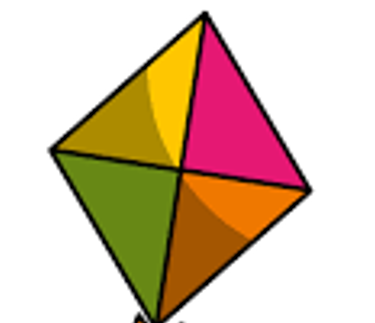
\includegraphics[height= 2.5cm, width= 3.5 cm]{C5M05 – DT – Q1.png}},
optionA={No sides},
optionB={Six sides},
optionC={Four sides},
optionD={Three sides},
correctoption={C},
leftmini={0.5},
rightmini={0.4},
}
% end-of-question

%-----------------------------------------------------------
%                        Question [  ]
%-----------------------------------------------------------
% start-of-question
\mcqimgleftFourOne{
questionnumber={17}, 
questionTag={C5M05 – DT – Q2},  
questiontext={Find the length of pencil. },
imgtabletikz = { 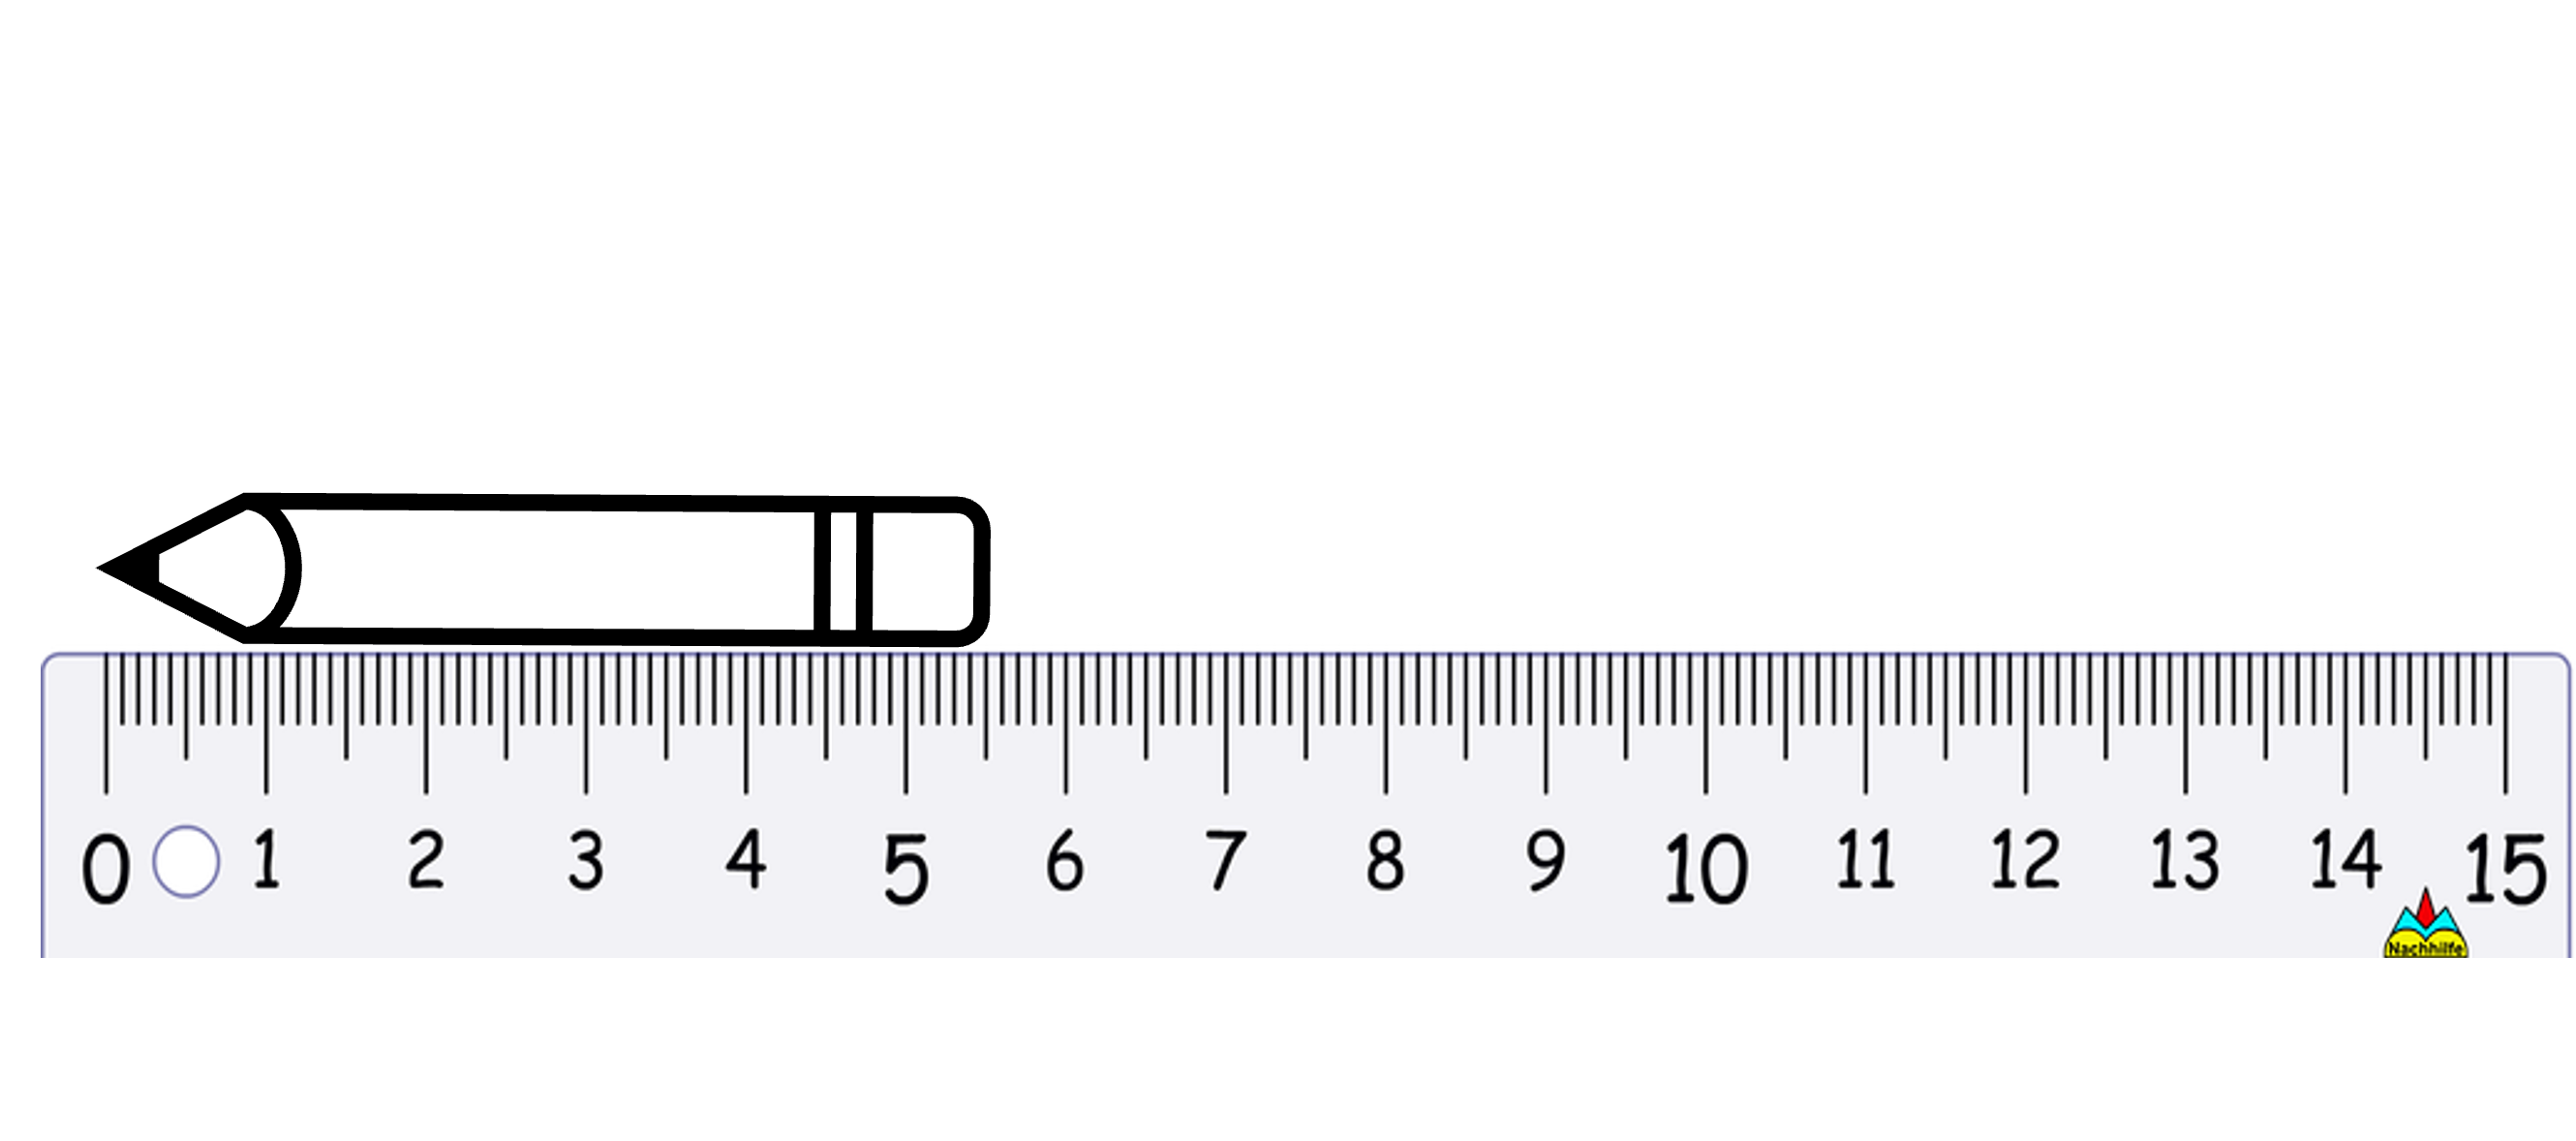
\includegraphics[height= 3cm, width= 10 cm]{C5M05 – DT – Q2.png}},
optionA={6.5 cm},
optionB={5.5 cm},
optionC={5 cm},
optionD={6 cm},
correctoption={B},
leftmini={0.6},
rightmini={0.3},
}
% end-of-question

%-----------------------------------------------------------
%                        Question [  ]
%-----------------------------------------------------------
% start-of-question
\mcqimgleftFourOne{
questionnumber={18}, 
questionTag={C5M05 – DT – Q3},  
questiontext={In the given figure, the angle formed is \rule{80pt}{0.5pt} the right angle. },
imgtabletikz = { 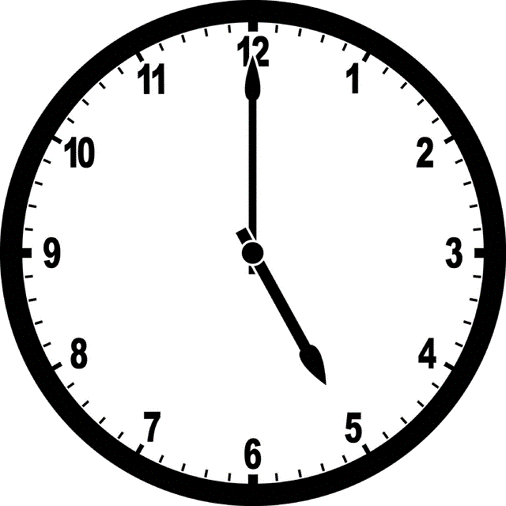
\includegraphics[height= 3cm, width= 3 cm]{C5M05 – DT – Q3.png}},
optionA={Equal to},
optionB={Greater than},
optionC={Lesser than},
optionD={Not equal to},
correctoption={B},
leftmini={0.6},
rightmini={0.3},
}
% end-of-question

%-----------------------------------------------------------
%                        Question [  ]
%-----------------------------------------------------------
% start-of-question
\mcqimgleftFourOne{
questionnumber={18}, 
questionTag={C5M08 – DT – Q1},  
questiontext={Find the area of the following shaded squares, if the side of one square is 1 cm. },
imgtabletikz = { 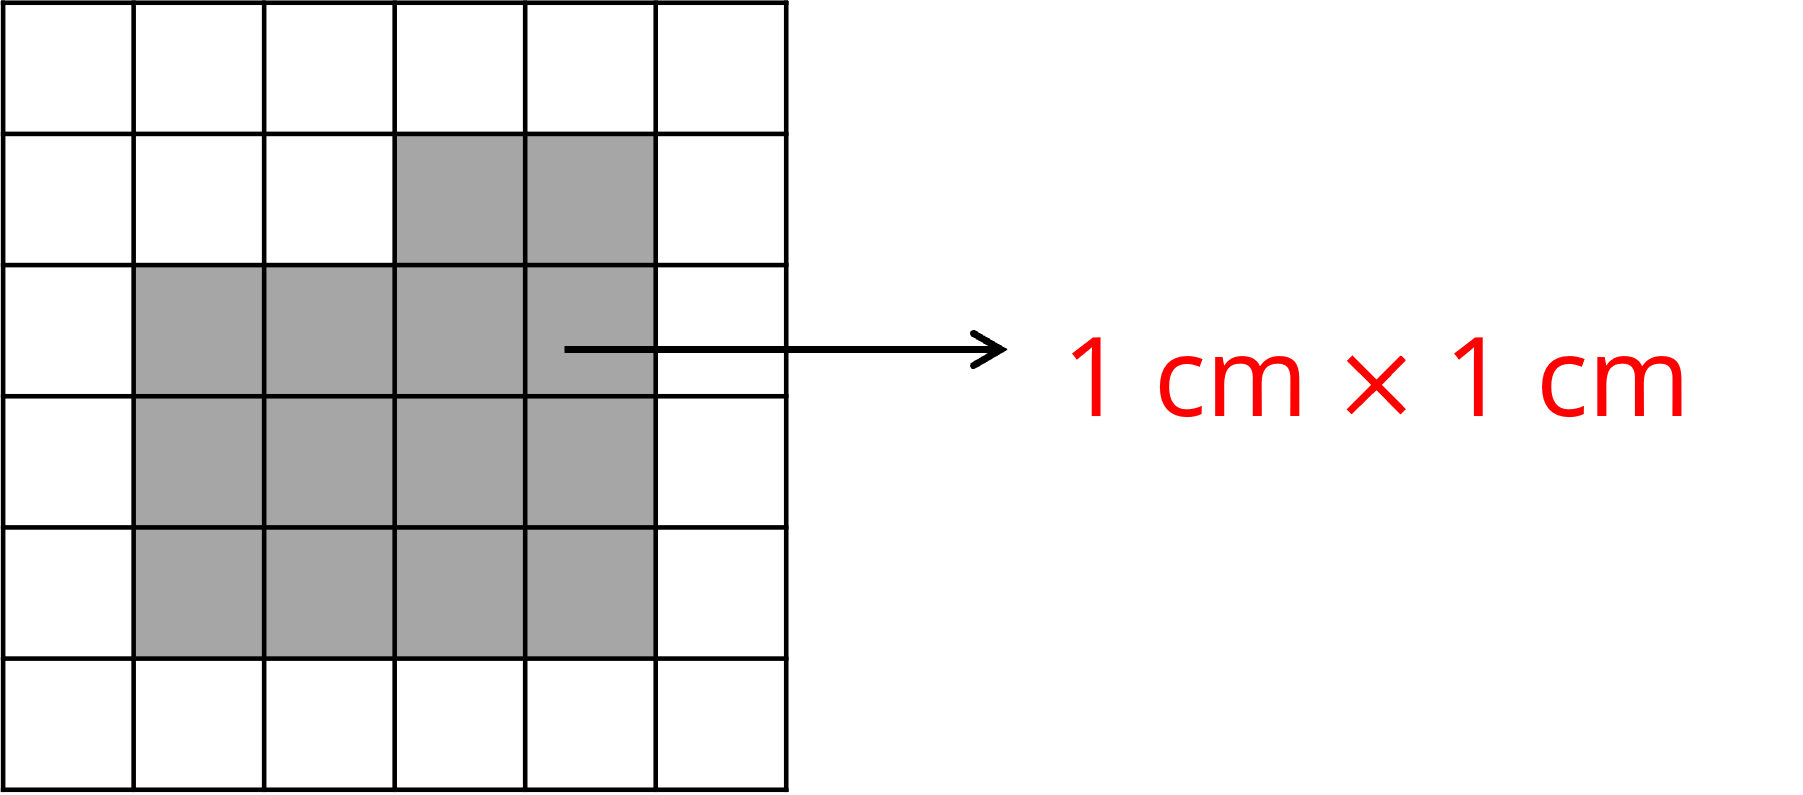
\includegraphics[height= 2.5cm, width= 6 cm]{C5M08 – DT – Q1.png}},
optionA={28 sq. cm},
optionB={56 sq. cm},
optionC={14 sq. cm},
optionD={7 sq. cm},
correctoption={C},
leftmini={0.6},
rightmini={0.3},
}
% end-of-question

%-----------------------------------------------------------
%                        Question [  ]
%-----------------------------------------------------------
% start-of-question
\mcqtextbottomOneFour{
questionnumber={19}, 
questionTag={C5M08 – DT – Q2},  
questiontext={Find the perimeter of the rectangle if its length and breadth is 10 cm and 4 cm respectively. },
optionA={14 cm},
optionB={28 cm},
optionC={40 cm},
optionD={104 cm},
correctoption={B},
}
% end-of-question

%-----------------------------------------------------------
%                        Question [  ]
%-----------------------------------------------------------
% start-of-question
\mcqimgleftFourOne{
questionnumber={20}, 
questionTag={C5M08 – DT – Q3},  
questiontext={Find the area of the rectangle. },
imgtabletikz = { 
\tikzset{every picture/.style={line width=0.75pt}} 
\begin{tikzpicture}[x=0.75pt,y=0.75pt,yscale=-1,xscale=1]
\draw  [fill={rgb, 255:red, 155; green, 155; blue, 155 }  ,fill opacity=0.48 ] (122,102) -- (294,102) -- (294,179) -- (122,179) -- cycle ;
\draw (186,80) node [anchor=north west][inner sep=0.75pt]   [align=left] {20 cm};
\draw (299,127) node [anchor=north west][inner sep=0.75pt]   [align=left] {8 cm};
\end{tikzpicture} },
optionA={12 sq. cm},
optionB={28 sq. cm},
optionC={56 sq. cm},
optionD={160 sq.cm},
correctoption={D},
leftmini={0.6},
rightmini={0.3},
}
% end-of-question

%-----------------------------------------------------------
%                        Question [  ]
%-----------------------------------------------------------
% start-of-question
\mcqtextbottomOneFour{
questionnumber={21}, 
questionTag={C5M07 – DT – Q1},  
questiontext={Which of the following letter look same after half a turn? },
optionA={N},
optionB={S},
optionC={O},
optionD={L},
correctoption={C},
}
% end-of-question

%-----------------------------------------------------------
%                        Question [  ]
%-----------------------------------------------------------
% start-of-question
\mcqtextbottomOneFour{
questionnumber={21}, 
questionTag={C5M07 – DT – Q2},  
questiontext={Pick the shape which is not divided into two mirror halves by the dotted line.\\
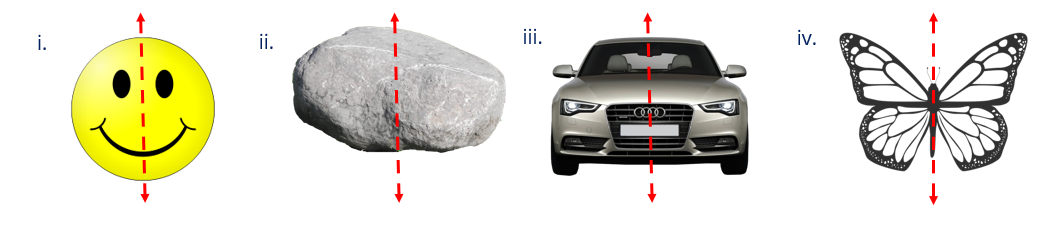
\includegraphics[height= 3.5cm, width= 16 cm]{C5M07 – DT – Q2.png}
},
optionA={i},
optionB={ii},
optionC={iii},
optionD={iv},
correctoption={B},
}
% end-of-question

%-----------------------------------------------------------
%                        Question [  ]
%-----------------------------------------------------------
% start-of-question
\mcqtextbottomOneFour{
questionnumber={22}, 
questionTag={C5M06 – DT – Q1},  
questiontext={Ajaykanth got a salary of Rs.10,000 in January month, Rs.12,000 in February month, Rs. 14,000 in March month and the pattern continued. How much he had earned in the month of June? },
optionA={Rs. 18,000},
optionB={Rs. 16,000},
optionC={Rs. 15,000},
optionD={Rs. 20,000},
correctoption={D},
}
% end-of-question

%-----------------------------------------------------------
%                        Question [  ]
%-----------------------------------------------------------
% start-of-question
\mcqimgleftFourOne{
questionnumber={23}, 
questionTag={C5M06 – DT – Q2},  
questiontext={ Identify the shape of the following image.},
imgtabletikz = { 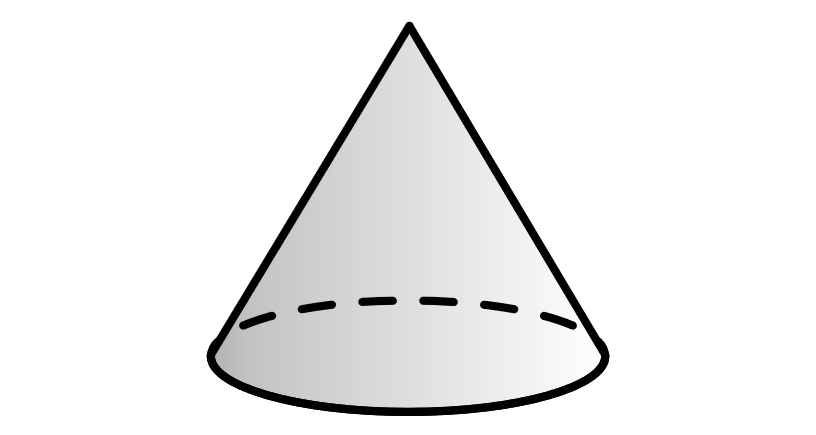
\includegraphics[height= 2.5 cm, width= 5 cm]{C5M06 – DT – Q2.png}},
optionA={Cube},
optionB={Cuboid},
optionC={Cone},
optionD={Cylinder},
correctoption={C},
leftmini={0.6},
rightmini={0.3},
}
% end-of-question

%-----------------------------------------------------------
%                        Question [  ]
%-----------------------------------------------------------
% start-of-question
\mcqtextbottomOneFour{
questionnumber={24}, 
questionTag={C5M09 – DT – Q1},  
questiontext={Find the number for the tally mark representation of \tikzset{every picture/.style={line width=0.75pt}} 
\begin{tikzpicture}[x=0.75pt,y=0.75pt,yscale=-1,xscale=1] 
\draw    (98.33,161.14) -- (98.33,183.39) ;
\draw    (110.28,161) -- (110.28,183.25) ;
\draw    (121.36,161.28) -- (121.36,183.53) ;
\draw    (133.31,161.42) -- (133.31,183.67) ;
\draw    (133.31,161.42) -- (98.33,183.39) ;
\draw    (145.26,161) -- (145.26,183.25) ;
\end{tikzpicture} },
optionA={8},
optionB={6},
optionC={7},
optionD={5},
correctoption={B},
}
% end-of-question

%-----------------------------------------------------------
%                        Question [  ]
%-----------------------------------------------------------
% start-of-question
\mcqimgleftFourOne{
questionnumber={25}, 
questionTag={C5M09 – DT – Q2},  
questiontext={Which genre is liked more? },
imgtabletikz = { 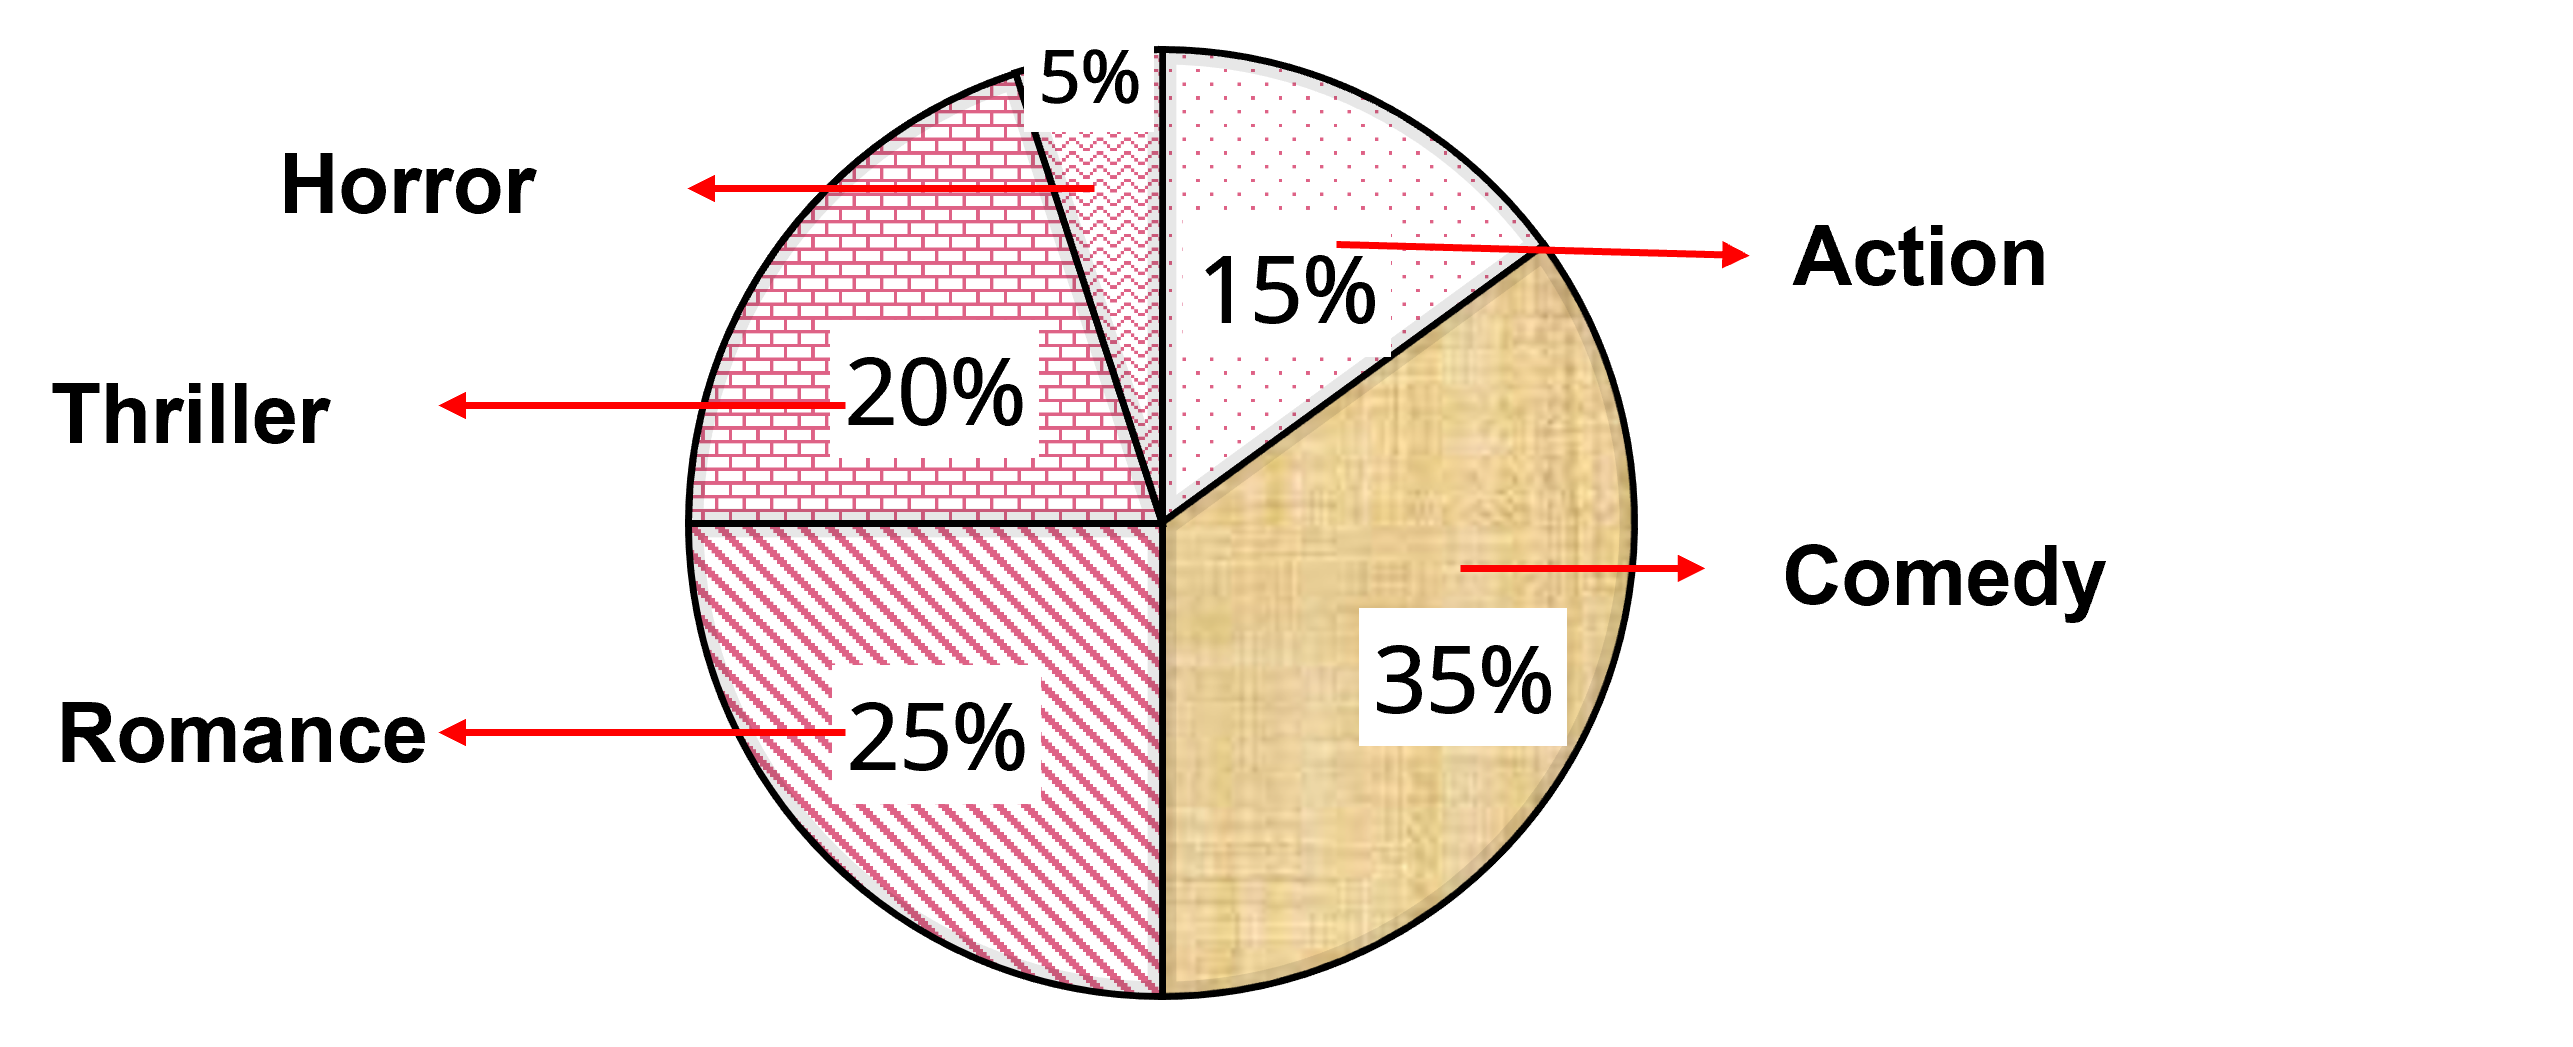
\includegraphics[height= 4cm, width= 10 cm]{C5M09 – DT – Q2.png}},
optionA={Comedy},
optionB={Horror},
optionC={Thriller},
optionD={Romance},
correctoption={A},
leftmini={0.6},
rightmini={0.3},
}
% end-of-question

\end{document}